% Mirror: https://github.com/SIGma-UIUC/presentation-format
% --------------------------------------------------------------------
% This is a simple Beamer document that uses beamerthemesigma.sty
% Reading the comments should help you create a presentation even if
% you've never used Beamer before.
% --------------------------------------------------------------------

% Set our document class to Beamer
\documentclass[aspectratio=169]{beamer}
% \documentclass[aspectratio=169, handout]{beamer}
% Add handout option to ignore pauses

% From Jeff E
\usepackage{algo}
\usepackage{sigmastyle}
\usepackage{mathdots}

\setbeamertemplate{blocks}[rounded]
\usecolortheme{orchid}
\usetheme{sigma}

% Set a title
\title{Dynamics and Chaos}

% Whoever worked on the presentation:
\author{Hanyang Sha}

% Date looks ugly, so leave blank
\date{12-02-2024}

% An institute name, if you're so inclined
% \institute{University of Illinois Urbana-Champaign}

% Use the SIGma theme for this Beamer presentation
\usetheme{sigma}
% --------------------------------------------------------------------

% Begin document
\begin{document}

% Beamer calls each slide a "frame", defined within the environment:
% \begin{frame}
%   <frame content here>
% \end{frame}

% This frame is just the title.
\begin{frame}
\titlepage
\end{frame}

% A frame with the table of contents.
% This frame's title is "Outline".
\begin{frame}{Outline}
  \tableofcontents
\end{frame}

\section{A Motivating Example}
\frame{\sectionpage}

\begin{frame}{Damped Driven Pendulum}
    Newton's Second Law for the damped driven pendulum: $$\ddot{\theta} + \gamma \dot{\theta} + \omega_0^2 \sin\theta = f \cos(\omega t),$$ where $\omega_0^2 = \frac{g}{l}$ and $f = \frac{F}{ml}$.\\\\
    We can nondimensionalize (via the Buckingham $\Pi$ theorem) the differential equations using the following: \\
    \begin{cases}
        $$t \coloneqq \omega_0 t$$ \\
        $$\frac{1}{q} \coloneqq \gamma/\omega_0$$ \\ 
        $$f \coloneqq f/\omega_0^2$$ \\ 
        $$\omega \coloneqq \omega/\omega_0$$
    \end{cases}, which gives $\ddot{\theta} + \frac{1}{q} \dot{\theta} + \sin\theta = f \cos(\omega t).$
\end{frame}

\begin{frame}{A Small Angle Approximation}
\begin{itemize}
    \item For small $\theta$, $\sin\theta \approx \theta$, so the differential equation becomes $\ddot{\theta} + \frac{1}{q} \dot{\theta} + \theta = f \cos(\omega t).$
    \item We know that the solution to this differential equation is the sum of a transient solution that depends on initial conditions and a steady state solution that is independent of initial solutions. 
\end{itemize}
\end{frame}

\section{Formal Theory}
\frame{\sectionpage}

\begin{frame}{Definitions}
    \begin{defn}
        $(X,d)$ metric space. $f:X\rightarrow X$. 
        \begin{enumerate}
            \item A \textbf{fixed point} $x\in X$ is a point s.t. $f(x)=x$. 
            \item A \textbf{periodic point} $x \in X$ is a point s.t. $\exists n\in\mathbb{N} : f^n(x)=x$, where the least such $n$ is called the \textbf{prime period}. 
            \item The \textbf{orbit} of $x$ under $f$ (denoted $O_f(x)$) is the sequence $x, f(x),\cdots,f^n(x),\cdots$ if $f$ not invertible or $\cdots, f^{-1}(x), x, f(x),\cdots$ if $f$ invertible. 
        \end{enumerate}
    \end{defn}  
\end{frame}

\begin{frame}{Definitions (cont.)}
    \begin{defn}
        $f:X\rightarrow X$ \textbf{exhibit sensitive dependence on initial conditions} if $\exists \delta > 0$ s.t. $\forall x \in X, \epsilon>0 \exists y\in X, N\in \mathbb{N} : x\neq y, d(x,y)<\epsilon, d(f^N(x),f^N(y)) \geq \delta$.
    \end{defn}
    Rmk. If a system possesses sensitive dependence, then numerical computation becomes invalid, because the inaccuracies of numerical computation become amplified. The true orbit may diverge from the computed orbit.
\end{frame}

\begin{frame}{Topological Transitivity}
    \begin{defn}
        $f:X\rightarrow X$ is \textbf{topologically transitive} if $\exists x\in X$ s.t. $O_f(x)$ is dense in $X$. 
    \end{defn}
    \begin{prop}
        If $X$ has no isolated points, $f:X\rightarrow X$ continuous, then $f$ topologically transitive is equivalent to the following: for nonempty open sets $U, V \subset X$, then $\exists N\in\mathbb{N} : f^N(U) \cap V \neq \emptyset$.
    \end{prop}
    Rmk. Reverse direction is obvious (consider contrapositive). The following is a proof of the forward direction. 
\end{frame}

\begin{frame}{Proof of Proposition (optional)}
    \begin{pf}
        $\because f$ topologically transitive $\therefore\exists n,m\in\mathbb{Z}:f^n(x)\in U, f^m(x)\in V$. Note that $f^n(x)\in U \rightarrow x\in f^{-n}(U) \rightarrow f^m(x) \in f^{m-n}(U),$ hence $f^m(x) \in f^{m-n}(U) \cap V \neq \emptyset$. If $m>n$, we are done since $m-n\in \mathbb{N}$.
        Suppose $\nexists m>n:f^m(x)\in V$. Then there exists decreasing sequence $(n_k)_{k=1}^\infty \subset \mathbb{Z}$ s.t. 
        \begin{enumerate}
        \item $n_k \leq n \forall k$
        \item $n_k \rightarrow -\infty$ as $k\rightarrow \infty$
        \item $f^{n_k}(x)\in V \forall k$ by denseness of $O_f(x)$ in $X$
        \item $f^{n_k}(x) \rightarrow f^m(x)$ as $k\rightarrow \infty$
        \end{enumerate}
        $\because f^m(x) \in f^{m-n}(U) \therefore$ by (4) $\exists m' \in (n_k) : m' < 2m-n, f^{m'}(x) \in f^{m-n}(U)$. Pick $x':=f^{n-m}(f^{m'}(x)) \in f^{n-m}(f^{m-n}(U))=U$. Then $f^{2m-n-m'}(x')=f^m(x)\in V$. Take $N=2m-n-m'\in \mathbb{N}$. Then $x'\in U\rightarrow f^N(x')\in f^N(U)$, and $f^N(x')\in V$, hence $f^N(U) \cap V \neq \emptyset$. $\blacksquare$
        
    \end{pf}
\end{frame}

\begin{frame}{Chaos}
    \begin{defn}[Devaney]
        $f:X\rightarrow X$ continuous. $f$ is \textbf{chaotic} if it is topologically transitive and its periodic points are dense. 
    \end{defn}
    \begin{thrm}
        Chaotic maps exhibit sensitive dependence on initial conditions, unless the entire space consists of a single periodic orbit. 
    \end{thrm}
   Rmk. The converse to the theorem is not true. A common misunderstanding is that chaotic is equivalent to sensitive dependence on initial conditions. But this is obviously false from definition of chaotic. 
\end{frame}

\begin{frame}{Proof of Theorem (Optional)}
    \begin{pf}
        We will prove sensitive dependence for $\epsilon \in (0,\delta)$. Then the case $\epsilon\geq\delta$ follows immediately. \\\\
        Unless the entire space consists of only a single periodic orbit, denseness of periodic points implies that there exists at least 2 distinct periodic orbits. Because periodic orbits are disjoint, $\exists p, q$ on separate periodic orbits s.t. $\delta := \frac18\displaystyle\min_{n,m\in\mathbb{Z}}(d(f^n(p),f^m(q)) > 0$. We claim $\delta$ works. \\\\
        Obs. Fix $x\in X$. Then the orbit of either $p$ or $q$ is always at least a distance of $4\delta$ from $x$. WLOG this point is q.\\\\
        Take $V:= \displaystyle\bigcap_{i=0}^n f^{-i}(B_\delta^o(f^i(q))).$  By previous proposition, $\exists k\in \mathbb{N}:f^k(B_\epsilon^o(x))\cap V\neq \emptyset \rightarrow \exists y\in B_\epsilon^o(x): f^k(y)\in V$. 
    \end{pf}
\end{frame}

\begin{frame}{Proof of Theorem (cont.)}
    \begin{pf}
        Suppose $p\in B_\epsilon^o(x)$ and has period $n$. Consider $N := n(\lfloor\frac{k}{n}\rfloor+1) \rightarrow 0 < N-k \leq n$. \\\\
        By triangle inequality: $d(f^N(p),f^N(y)) = d(p,f^N(y)) \geq d(x,f^{N-k}(q)) - d(f^{N-k}(q),f^N(y)) - d(p,x) \geq 4\delta -\delta -\delta = 2\delta$, because $p\in B_\epsilon^o(x) \subset B_\delta^o(x)$ and $f^N(y) \in f^{N-k}(V) \subset B_\delta^o(f^{N-k}(q))$ (take $i=N-k$ in definition of $V$). \\\\
        Thus, either $d(f^N(p),f^N(x)) \geq \delta$ or  $d(f^N(y),f^N(x)) \geq \delta$. \\\\
        Recall that $d(p,x)<\epsilon$ and $d(y,x)<\epsilon$. $\blacksquare$
    \end{pf}
\end{frame}

\begin{frame}{Example of Chaotic Mapping}
    Consider $f:[-2,2]\rightarrow [-2,2], x \mapsto 2|x|-2$. 
\begin{itemize}
    \item Denseness of periodic points: we can always find subinterval $I$ of length $1/2^{n-2}$ s.t. $f^n(I) = [-2,2].$ Thus, $f^n$ has a fixed point on $I$.
    \item Topological transitivity: $\forall U\subset [-2,2], \exists n\in\mathbb{N} : f^n(U) = [-2,2]$. Then $\forall V\subset [-2,2], f^n(U) \cap V \neq\emptyset.$ 
\end{itemize}
\end{frame}

\section{Lyapunov Exponent}
\frame{\sectionpage}

\begin{frame}{Definition}
    \begin{defn}[Discrete System]
        $f:X\rightarrow X$. Let $x,y$ be initial points in the phase space. The separation vector $\delta(n)$ is given by $\delta(n) = f^n(x)-f^n(y)$. The \textbf{Lyapunov exponent} $\lambda$ is defined as $$\lambda = \displaystyle \lim_{n\rightarrow \infty} \lim_{||\delta(0)||\rightarrow 0} \frac{1}{n} \ln{\frac{||\delta(n)||}{||\delta(0)||}}.$$
    \end{defn}
    \begin{defn}[Continuous System]
        $f:\mathbb{R}\rightarrow X$. Let $x,y$ be two trajectories in the phase space. The separation vector $\delta(t)$ is given by $\delta(t) = x(t)-y(t)$. The \textbf{Lyapunov exponent} $\lambda$ is defined as $$\lambda = \displaystyle \lim_{t\rightarrow \infty} \lim_{||\delta(0)||\rightarrow 0} \frac{1}{t} \ln{\frac{||\delta(t)||}{||\delta(0)||}}.$$
    \end{defn}
\end{frame}

\begin{frame}{Remarks}
    \begin{itemize}
        \item Intuitively, this means that (for a discrete system) for $n$ large, $||f^n(x+\delta)-f^n(x)|| \approx \delta e^{\lambda n}$. 
        \item The Lyapunov Exponent measures the rate at which two initially extremely close states grow over time.
        \item If $\lambda > 0$, the distance between the two states grows over time, and is a good indicator of chaotic systems.
        \item From this, it is obvious that $\lambda>0$ implies that $f$ has sensitive dependence on initially conditions.
        \item However, $\lambda>0$ does not \textit{necessarily} imply chaos. Additional information regarding the system is needed. 
    \end{itemize}
\end{frame}

\begin{frame}{Maximal Lyapunov Exponent}
    \begin{itemize}
        \item $\lambda$ may be different for different initial separation vectors $\delta(0)$, creating a spectrum.
        \item For example, consider the first order linear system $\vec{x}'=A\vec{x}+\vec{f}(t)$, with $A$ constant. From differential equations, we can observe that real parts of eigenvalues of $A$ are Lyapunov exponents. 
        \item We define the \textbf{maximal Lyapunov exponent} as the largest value in the spectrum. 
    \end{itemize}
\end{frame}

\begin{frame}{A Practical Formulation}
\begin{itemize}
    \item From $\left|f^n(x+\delta)-f^n(x)\right| \approx \delta e^{\lambda n}$, isolate $\lambda$: $\lambda \approx \frac{1}{n} \ln{\left|\frac{f^n(x+\delta)-f^n(x)}{\delta}\right|}$. \\
    \item Take $\delta \rightarrow 0$, we apply definition of a derivative: $\lambda\approx\frac{1}{n}\ln{\left|(f^n(x))^\prime\right|}.$\\
    \item Using chain rule: $(f^n(x))^\prime = f^\prime(f^{n-1}(x)) \cdot f^\prime(f^{n-2}(x)) \cdots f^\prime(f(x)) \cdot f^\prime(x)=\displaystyle \prod_{i=0}^{n-1} f^\prime(x_i),$
    where $x_i := f^{i}(x)$. Substitute in $(f^n(x))^\prime$: $\lambda\approx\displaystyle\frac{1}{n}\ln{\left| \prod_{i=0}^{n-1} f^\prime(x_i)\right|}.$\\
    \item Take $n \rightarrow \infty$: $\lambda=\displaystyle \lim_{n\to\infty}\frac{1}{n}\ln{\left| \prod_{i=0}^{n} f^\prime(x_i)\right|}=\displaystyle\lim_{n\to\infty} \frac{1}{n}\sum_{i=0}^{n}\ln{\left|  f^\prime(x_i)\right|}.$\\
    \item For continuous systems, an equivalent formulation is $\lambda = \int f(x)\ln{\left|  f^\prime(x)\right|}dx.$
\end{itemize}
\end{frame}

\begin{frame}{Example}
    \begin{itemize}
        \item Consider the doubling map on the unit circle: $D:S^1\rightarrow S^1$ (equivalently $D:[0,2\pi)\rightarrow[0,2\pi)$), $\theta \mapsto 2\theta \mod 2\pi$, where $S^n$ denotes the unit sphere in $(n+1)$-dimensional Euclidean space.
        \item $D'(\theta)=2 \forall \theta \neq \pi$. We can ignore the discontinuity at $\theta = \pi$. 
        \item Hence, $\lambda =\displaystyle\lim_{n\to\infty} \frac{1}{n}\sum_{i=0}^{n}\ln{\left| f^\prime(x_i)\right|} = \displaystyle\lim_{n\to\infty} \frac{1}{n}\sum_{i=0}^{n}\ln2 = \ln2 > 0$, meaning $D$ has sensitive dependence on initial conditions. 
        \item Exercise: prove that $D$ is chaotic. 
    \end{itemize}
\end{frame}

\section{Bifurcations}
\frame{\sectionpage}

\begin{frame}{Attraction and Repulsion}
    \begin{defn}
        A fixed point $x_0$ is \textbf{attracting/stable} if $\exists \lambda \in (0,1)$ and open interval $U$ containing $x_0$ s.t. $|f(x)-f(x_0)|=|f(x)-x_0| \leq \lambda|x-x_0| \forall x\in U$. Similarly, $x_0$ is \textbf{repelling/unstable} if $\exists \lambda>1$ and open interval $U$ containing $x_0$ s.t. $|f(x)-x_0| \geq \lambda|x-x_0| \forall x\in U$. 
    \end{defn}
    Rmk. It follows from the definition of attraction that $O_f(x) \rightarrow x_0 \forall x \in U$.
    \begin{defn}
        A periodic point of period $n$ is attracting (repelling) if it is an attracting (repelling) fixed point of $f^n$. 
    \end{defn}
\end{frame}

\begin{frame}{A Practical Formulation}
    \begin{thrm}
        $f:X\rightarrow X$ differentiable at fixed point $x_0 \in X$. Let $a := |f'(x_0)|$. Then: 
        \begin{enumerate}
            \item $x_0$ is attracting iff $a<1$. 
            \item $x_0$ is repelling iff $a>1$. 
        \end{enumerate}
    \end{thrm}
    \begin{pf}
        We will prove $(1)$. The proof of $(2)$ is similar. \\
        $(\leftarrow) \because a = f'(x_0) \therefore \forall \epsilon >0 \exists \delta >0 : 0<|x-x_0|<\delta \rightarrow |\frac{f(x)-f(x_0)}{x-x_0}| \in (a-\epsilon, a+\epsilon)$. Take $\epsilon < 1-a$ and $U = (x_0-\delta, x_0+\delta)$. \\
        $(\rightarrow)$ Consider contrapositive: $a\geq 1 \rightarrow$ not attracting. 
    \end{pf}
\end{frame}

\begin{frame}{Bifurcation}
\begin{itemize}
    \item Let $\lambda$ be a external parameter. Let $f:X\rightarrow X$ be a function dependent on $\lambda$. Varying $\lambda$ generates a family of functions, denoted $f_\lambda$, where each function in the family uses a different value of $\lambda$. 
    \item As we change $f$ by varying $\lambda$, there are certain points in the family where the qualitative behavior of the function changes. These changes are called \textbf{bifurcations}, and the values of the parameter $\lambda$ where these changes occur are called \textbf{bifurcation points}.
\end{itemize}
\end{frame}

\begin{frame}{Theorem: No Bifurcation}
\begin{thrm}
    Let $f_\lambda$ be a family of functions. Suppose $f_{\lambda_0}(x_0)=x_0$ and $f'_{\lambda_0}(x_0) \neq 1$. Then $\exists$ interval $I$ s.t. $x_0 \in I$, interval $N$ s.t. $\lambda_0 \in N$, and continuously differentiable function $p: N\rightarrow I$ s.t. $p(\lambda_0) = x_0$ and $f_\lambda(p(\lambda)) = p(\lambda)$. Moreover, $f_\lambda$ has no other fixed points in $I$.
\end{thrm}
\begin{pf}
    Consider function $g(x,\lambda) = f_\lambda(x)-x$. We have $g(x_0, \lambda_0)=0$, $\frac{\partial g}{\partial x}(x_0,\lambda_0) = f'_{\lambda_0}(x_0)-1 \neq 0$. Apply the implicit function theorem on $g$ at $(x_0, \lambda_0)$.
\end{pf}
\end{frame}

\begin{frame}{Period Doubling Bifurcation: Definition}
\begin{defn}
    A family of functions $f_\lambda$ undergoes a \textbf{period doubling bifurcation} at $\lambda = \lambda_0$ if $\exists$ open interval $I$, $\epsilon >0$ s.t.: 
    \begin{enumerate}
        \item $\forall \lambda \in [\lambda_0-\epsilon, \lambda_0+\epsilon], \exists !$ fixed point $p_\lambda \in I$ for $f_\lambda$.
        \item $\forall \lambda \in (\lambda_0-\epsilon, \lambda_0], f_\lambda$ has no cycles of period 2 in $I$ and $p_\lambda$ is attracting (resp. repelling). 
        \item $\forall \lambda \in (\lambda_0, \lambda_0+\epsilon), \exists !$ 2-cycle $q_\lambda^1, q_\lambda^2$ in $I$ that is attracting (resp. repelling). Meantime, fixed point $p_\lambda$ is repelling (resp. attracting). 
        \item As $\lambda\rightarrow\lambda_0$, $q_\lambda^i \rightarrow p_{\lambda_0}$.
    \end{enumerate}
\end{defn}
\end{frame}

\section{A Second Look at Damped Driven Pendulum}
\frame{\sectionpage}

\begin{frame}{Spontaneous Symmetry Breaking Bifurcation}
$$\ddot{\theta} + \frac{1}{q} \dot{\theta} + \sin\theta = f \cos(\omega t).$$
\begin{itemize}
    \item Note that the pendulum equation is invariant under the transformation $\theta \mapsto -\theta, t \mapsto t-\pi/\omega$. Thus, if $\theta_1(t)$ is a solution, then $\theta_2(t) = -\theta_1(t-\pi/\omega)$ is also a solution. 
    \item Physically, this means that the equations make no distinction between the left and right sides of the vertical $\theta = 0$. 
    \item We say the solution is \textit{symmetric} if $\theta_1(t) = \theta_2(t)$; otherwise, \textit{spontaneous symmetry breaking} has occurred. This symmetry breaking produces an additional loop on the phase diagram. \\
\end{itemize}
\end{frame}

\begin{frame}{Spontaneous Symmetry Breaking Bifurcation (cont.)}
\begin{itemize}
    \item At $q \approx 1.246$, the symmetry is broken. 
    \item For $q < 1.246$, the asymptotic solution (limit cycle) is symmetric. 
    \item For $q > 1.246$, there exists a pair of stable, asymmetric asymptotic solutions. The original limit cycle still exists but becomes unstable. Depending on initial conditions, the trajectory converges to one of the stable limit cycles. 
    \item Demo!
\end{itemize}
\end{frame}

\begin{frame}{Period Doubling Bifurcation}
    Demo!
\end{frame}

\begin{frame}{Bifurcation Diagram}
\begin{enumerate}
    \item Find limit cycle for some $q$ and plot it in the 2D phase plane.
    \item Construct is a 1D subspace (called the \textit{Poincare section}) of the 2D phase plane.
    \item Take the intersection of the limit cycle and the Poincare section.
    \item Plot data points where $q$ is the x coordinate and $\theta$ is y coordinate.  
\end{enumerate}
\end{frame}

\begin{frame}{Very Scuffed Bifurcation Diagram that I drew}
    \begin{figure}[htp]
        \centering
        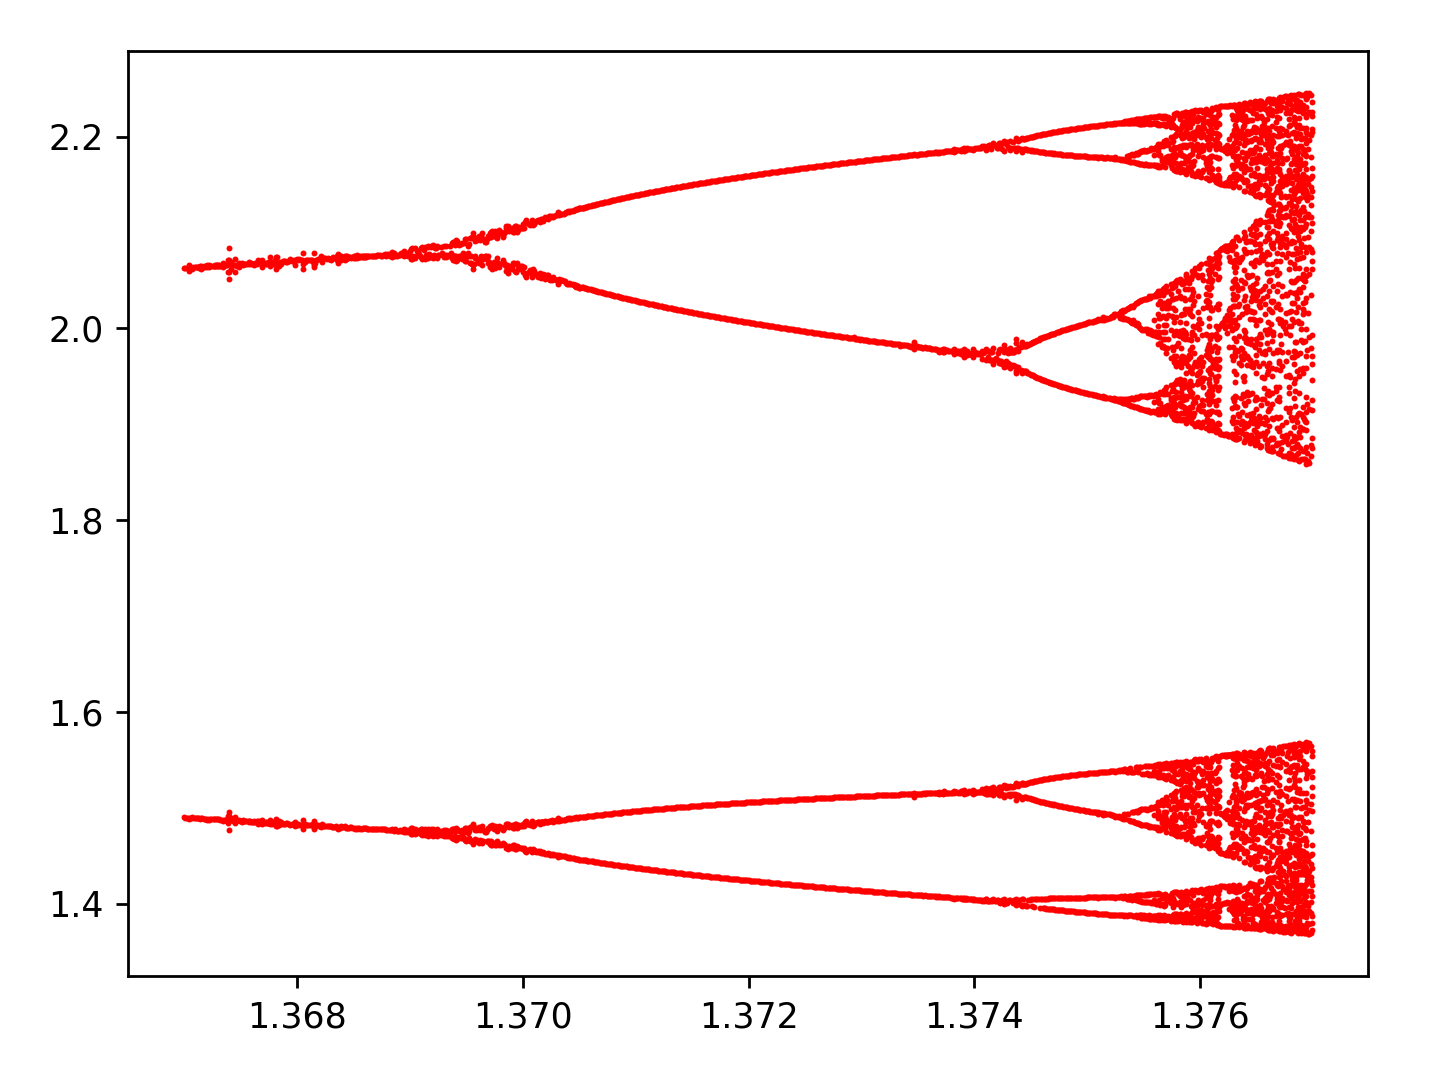
\includegraphics[width=7cm]{images/bifurcation.png}
        \caption{\textbf{Bifurcation Diagram of the Damped Driven Pendulum} with $f = 1,5$, $\omega = 2/3$, and $1.367 < q < 1.377$.}
        \label{fig:Bifurcation}
    \end{figure}
\end{frame}

\section{A Classic Example: Logistic Map}
\frame{\sectionpage}

\begin{frame}{Definition}
    A 1D map can be expressed in the form of $x_{n+1} = f(x_n)$. 
    \begin{defn}
        The \textbf{logistic map} is a family of functions $f\mu: \mathbb{R}\rightarrow \mathbb{R}, x \mapsto \mu x(1-x),\mu\in\mathbb{R}$.
    \end{defn}
    Specifically, we will investigate $\mu>0$.
\end{frame}

\begin{frame}{First Period Doubling Bifurcation}
\begin{itemize}
        \item Recall that fixed point $x_*$ is stable if $\lvert f'(x_*) \rvert < 1$ and unstable if $\lvert f'(x_*) \rvert > 1$. Bifurcations usually occur at the \textit{marginally stable} point of $\lvert f'(x_*) \rvert = 1$. 
    \item The initial fixed points for small $\mu$ are: $x = \mu x(1-x) \rightarrow x_* = 0, 1-1/\mu$. $f'_\mu = \mu(1-2x)$, so $x_* = 0$ is stable for $0 < \mu < 1$, and $x_* = 1-1/\mu$ is stable for $1 < \mu < 3$.
    \item At $\mu = 3$, $x_* = 1-1/3 = 2/3$, and $f'_\mu(x_*) = \mu(1-2x_*) = 3(1-2 \cdot 2/3) = -1$, which is a marginally stable point, causing the first bifurcation.
    \item The 2 periodic points (denoted $x_0$ and $x_1$) after the bifurcation must both satisfy $x = f_\mu(f_\mu(x)) = f_\mu^2(x)$, which is a quartic equation. Note that 2 roots are the initial fixed points $x_* = 0, 1-1/\mu$, so factor them out to get $ x_1, x_2 = \frac{1}{2\mu}(\mu+1 \pm \sqrt{(\mu+1)(\mu-3)})$.
\end{itemize}
\end{frame}

\begin{frame}{Subsequent Period Doubling Bifurcations}
\begin{itemize}
    \item To find the value of $\mu$ at which a bifurcation occurs (going from period-$2^{n-1}$ to period-$2^n$, we use $(f_\mu^{2^{n-1}})'(x_i) = -1$ for all fixed points $x_i$ of $f_\mu^{2^{n-1}}$. 
    \item Using the chain rule, $(f_\mu^{2^{n-1}})'(x_0) = f'_\mu(f^{2^{n-1}-1}_\mu(x_0))f'_\mu(f^{2^{n-1}-2}_\mu(x_0)) \cdots f'_\mu(f_\mu(x_0)) f'_\mu(x_0)$ $= f'_\mu(x_{2^{n-1}-1}) f'_\mu(x_{2^{n-2}-2}) \cdots f'_\mu(x_1) f'_\mu(x_0) = \displaystyle \prod_{i=0}^{2^{n-1}-1} f'_\mu(x_i) = \displaystyle \prod_{i=0}^{2^{n-1}-1} \mu(1-2x_i) = -1.$
    \item We know where the fixed points $x_i$ are for period-$2^{n-1}$, so we can solve the equation as a function in $\mu$.
\end{itemize}
\end{frame}

\begin{frame}{Feigenbaum Constant}
\begin{itemize}
    \item It turns out that if we take the ratio of the space between consecutive period doubling bifurcation points of the logistic map, we approach a value known as the Feigenbaum constant $\delta=4.669...$ (A006890 in OEIS). 
    \item Let $q_n$ be the value of $q$ of the $n$-th bifurcation. Let $\delta_n := \frac{q_{n+1} - q_n}{q_{n+2} - q_{n+1}}$. Then $\delta := \displaystyle \lim_{n \rightarrow \infty} \delta_n$. 
    \item This constant is \textit{universal} for all 1D maps with a single locally quadratic maximum. 
\end{itemize}
\end{frame}

% Asking questions is fun but we should answer some first
\begin{frame}{}
      \begin{center}
    {\color{sigma@mainblue} \LARGE Questions?}
  \end{center}
\end{frame}

\begin{frame}{Further Reading}
    \begin{itemize}
        \item Theorems for sufficient conditions of saddle node bifurcations and period doubling bifurcations
        \item Topological conjugacy and structural stability
        \item Sharkovsky's Theorem
        \item Fractal dimension of strange attractors
    \end{itemize}
\end{frame}

% Quotes are fun, find some to use!
\font\eightss=cmssq8
\font\eightssi=cmssqi8
\newcommand\quoteAuthorDate[3]{\begingroup
  \baselineskip 10pt
  \parfillskip 0pt
  \interlinepenalty 10000 % not needed in example
  \leftskip 0pt plus 40pc minus \parindent
  \let\rm=\eightss
  \let\sl=\eightssi
  \everypar{\sl}#1\par
  \nobreak\smallskip
  \noindent\rm--- #2\unskip\enspace(#3)\par
  \endgroup}
% If someone can figure out how to horizontally center this and make the text bigger that'd be cool
\begin{frame}
    \begin{center}
        \item \quoteAuthorDate{Chaos is lawless behavior governed entirely by law.}{Ian Stewart}{\textcolor{sigma@mainblue}{1989}}
    \end{center}
\end{frame}

% Remove this slide if you came up with all the material yourself
\begin{frame}[allowframebreaks]{Bibliography}
    \tiny
    \bibliography{refs}
    \bibliographystyle{alpha}
    \begin{itemize}
        \item Hasselblatt, Boris; Anatole Katok (2003). \textit{A First Course in Dynamics: With a Panorama of Recent Developments}. Cambridge University Press.
        \item Devaney, Robert (1989). \textit{A First Course in Chaotic Dynamical Systems}. CRC Press.
        \item Devaney, Robert (1989). \textit{An Introduction to Chaotic Dynamical Systems}. Addison-Wesley.
        \item Chasnov, Jeffery R (2013). \textit{Scientific Computing}. Hong Kong University of Science and Technology.
        \item Texas A&M University MATH 614 Spring 2016 lecture slides. 
    \end{itemize}
\end{frame}

\end{document}